\documentclass[12pt]{report}

\usepackage{graphicx}

\begin{document}
\title{Trabajo de Investigación:\\¿Cómo Funciona Kankan?}
\author{Garay Araujo Fernando Raúl}
\date{Diciembre del 2022}
\maketitle
\newpage

\section*{I. Introducción}

Con la llegada de las altas velocidades de transmisión por internet, una de las principales característcas en las que se intentó innovar e implementar es en la transmisión de archivos multimedia como son los videos.\\
Para satisfacer esta necesidad, han surgido diferentes plataformas en la web, algunas más conocidas que otras. Dentro de las conocidas en nuestro lado occidental del mundo tenemos a YouTube o a Netflix.\\
Sin embargo, para occidente también se encuentra esta necesidad y por temas políticos no le resulta conveniente a algunos de esos países tener empresas americanas funcionando en sus países ni siendo las más predominantes como lo han sido en nuestro lado del planeta.\\
Es aquí cuando una de las compañías del top 10 de las más grandes compañías chinas de internet entra en acción para satisfacer la necesidad de los chinos. Xunlei Limited, crea Kankan, actualmente una aplicación web de streaming de videos, originalmente con el propósito de ser un extra para su principal servicio allá por el 2007, un acelerador de archivos basado en P2P. Después de un poco tiempo, Kankan pasa de ser un extra de este acelerador y pasa a ser una plataforma individual e independiente (con su propio sitio web) de streaming de videos.\\
Debido a su alta popularidad es que es de nuestro interés el saber cómo funciona y cómo es que puede brindar estos servicios de manera efectiva a uno de los países más poblados y extensos del mundo. Es por eso que en esta breve investigación ahondaremos un superficialmente en los detalles técnicos de los protocolos usados en la transferencia de archivos multimedia por parte de los servidores de Kankan hacia los clientes, e incluso como veremos más a continuación, el compartir paquetes entre usuarios usando P2P.

\section*{II. Funcionamiento de Kankan con los Clientes}

Kankan funciona de una manera muy particular y hasta cierto punto original, ya que para ser una aplicación de streaming de videos, no funciona con una sóla arquitectura como quizás podríamos sospechar de otras plataformas de este estilo, Kankan utiliza un híbrido entre P2P y CDN.\\
Su funcionamiento entre estas dos arquitecturas está muy poco ligado, trabajan casi de forma independiente estas dos. Y a grandes rasgos, dejamos una imagen que explica cómo funciona el envío de la información de parte de Kankan (esta es la parte de la arquitectura CDN) hacia los clientes, así como la manera en que funciona el envío de chunks entre los pares, en este caso los clientes (esta siendo la parte de la arquitectura P2P).

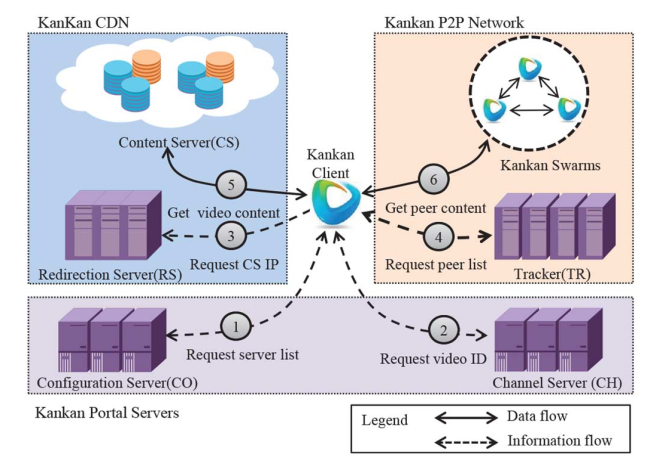
\includegraphics[height=10cm]{images/img1}.

Antes de explicar a detalle la imagen de las solicitudes de un cliente a Kankan, debemos hacer la observación de que una vez un cliente instala el cliente de Kankan, esta instalación asigna un mínimo de 2 GB que funcionará como almacenamiento de caché para transmitir entre pares en un futuro. Más adelante explicaremos un poco más a detalle cómo funciona esto.\\
Ahora, como podemos observar en la imaegn, el cliente primero hace una solicitud a los servidores de la plataforma de Kankan.\\
La primera solicitud sucede cuando se instala el cliente de Kankan, aquí se hace una solicitud hacia un servidor (Configuration Server o CO) cuya función es almacenar el dominio o direcciones IP de otros servidores de Kankan, los cuales nos darán los identificadores (los ID) de los videos que veremos en la plataforma. Entonces, instalando Kankan, tenemos las IP de los CO más cercanos a nuestro host.\\
Una vez navegando en la aplicación y seleccionamos un video, aquí estamos pidiendo a otro tipo de servidor, apodados Channel Servers (CH), los cuales almacenan el ID de los videos. Entonces seleccionando un video en la plataforma, el respectivo CH nos regresa el ID del video en cuestión que queremos ver, y nuestro cliente de Kankan también conoce la dirección de unos servidores, a los que apodaremos Redirection Servers (RS), los cuales nosotros les enviamos un ID de video y ellos nos regresan la IP de dos servidores parte de la CDN (apodados Primary/Secondary Content Server o PCS y SCS) que contienen parte de o el archivo del video completo en cuestión.\\
Aquí la cosa se pone interesante ya que hasta este punto estábamos viendo trabajar la parte de la arquitectura CDN de Kankan, pero aquí entra en juego la parte híbrida con P2P.\\
Tenemos el ID del video que queremos ver y la IP de los PCS y SCS que contienen el archivo de estos videos. Entonces, lo más lógico es solicitar a ambos servidores el contenido del video con el ID que tenemos, y en efecto es lo que hacemos (paso 5 en la imagen), pero mientras todo esto sucede, simultáneamente nos ponemos en comunicación con un Tracker para la asignación de una red de vecinos con los cuales vamos a intercambiar chunks del video. Aquí es donde entran en juego los 2GB reservados para caché de el cliente Kankan, ya que los pares usarán este espacio para compartirse chunks.\\
El Tracker nos asocia con nuestros vecinos mientras que el streaming de los primeros segundos de nuestro video son agilizados gracias a la conexión con los PCS y SCS, esto permite al cliente tener la experiencia de un arranque rápido de videos. Aunque el objetivo de tener P2P en este streaming es que poco a poco dejemos de cargar de solicitudes a los PCS y SCS y empecemos a depender un poco más en nuestros pares vecinos.\\
La razón por la que hay PCS y SCS, es porque el PCS tiene el archivo completo del video en cuestión, mientras que el SCS sólo tiene los primeros segundos del mismo. El disponer de dos CS para el arranque de la reproducción de un video nos ayuda muchísimo en mejorar la experiencia de usuario, ya que como decimos, se tiene un arranque rápido no recayendo en la esperanza de que los pares tengan los chunks necesarios para nuestro streaming.\\
Después de haber arrancado el video, se busca el soltar la dependencia en los CS, tratando de depender exclusivamente (mientras se pueda) en nuestros pares vecinos. Entonces tenemos un arranque CDN, y soltamos poco a poco la dependencia CDN para pasar a una forma híbrida entre CDN y P2P. Si podemos obtener todos los chunks de nuestro streaming por medio de P2P, pasamos a la arquitectura exclusiva P2P, pero si por alguna razón detectamos que en nuestro buffer no podemos obtener más de 10 segundos de reproducción futura de nuestro video, regresaremos a una arquitectura híbrida. Adjuntamos un gráfico que representa esta idea, en la cual pasamos de CDN exclusivo, a híbrido, luego P2P exclusivo y después se regresa a híbrido (y en general nunca se espera que siga un patrón exclusivo entre estas arquitecturas).

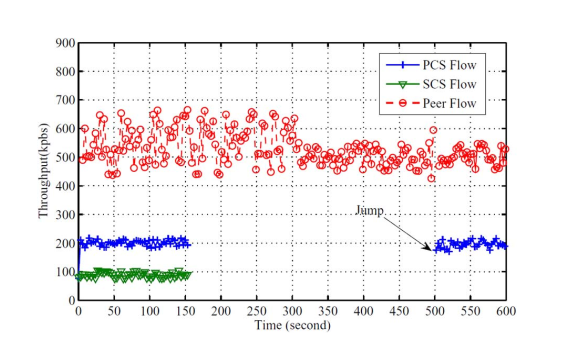
\includegraphics[height=10cm]{images/img2}.

Es importante destacar que, como podemos ver en el gráfico, si estamos en P2P exclusivo y necesitamos regresar a híbrido por falta de chunks en los pares, esta vez únicamente solicitaremos paquetes del CDN primario, o sea al SCS sólo lo utilizamos para el arranque del video.\\

Esta es básicamente la explicación del funcionamiento de la transferencia de archivos hacia los clientes siguiendo esta arquitectura híbrida entre CDN y P2P. Como podemos observar, estas arquitecturas en Kankan funcionan de manera prácticamente independiente.\\
La siguiente sección será para explicar brevemente los protocolos usados en la interacción con el Tracker y los SR.\\

\section*{III. Protocolos Usados en Kankan}

Nuestro propósito en esta sección es explicar y entender un poco a detalle los protocolos usados para la comunicación entre el cliente Kankan y los servidores o tracker, según corresponda, de Kankan.\\
Comenzaremos explicando el protocolo con los servidores de Kankan. Y es que teniendo el ID del video que queremos, le pedimos a los RS del cliente por medio de una GET/request del protocolo HTTP la dirección IP de los CS que tienen nuestro video. Para ser más específicos, nuestro cliente tiene asignados dos RS, el Primary y el Secondary (PRS y SRS). El PRS nos regresa un json, en el cual está la dirección IP y puerto del servidor el cual pasará a ser nuestro PCS exclusivamente, mientras que el SRS nos regresará un json con dos direcciones IP y sus respectivos puertos, uno de los cuales es el mismo que será nuestro PCS, y el segundo nuestro SCS (recordemos que exclusivamente para el arranque del streaming).\\
De la misma forma, la transferencia del video en sí con los CS, también es usando HTTP.\\
Entonces concluimos que el intercambio de información entre cliente Kankan y servidores Kankan por parte de la arquitectura CDN funciona con base en el protocolo HTTP.\\
Para la transferencia de archivos por la arquitectura P2P en Kankan funciona de una manera interesante, ya que por una parte la comunicación con el Tracker funciona con base en un protocolo (personalizado por Kankan el cual desconocemos a detalle) basado en TCP. Aquí no sólo le enviamos el ID del video, sino también una disperción de este ID el cual funciona como identificador del video en la respectiva red P2P. El tracker nos responderá con una lista (puede ser desde vacía hasta con cientos de entradas) en la cual cada entrada será un par de nuestra futura red, son tercias de la forma [ID del par, dirección IP, puerto].\\
Hasta aquí tenemos que la comunicación del cliente con el Tracker es usando una versión personalizada de TCP. Pero para la comunicación entre pares, es decir el compartir los chunks del contenido del video en sí, es usando una versión personalizada ahora de UDP.\\
En resumen, para la parte CDN de Kankan, funciona usando el protocolo HTTP, mientras que para la parte P2P funciona, con un protocolo basado en TCP para la comunicación con el tracker, y con protocolo basado en UDP para la comunicación entre pares.\\

\section*{IV. Servicios y Condiciones Ideales para Kankan}

Para el funcionamiento de Kankan, necesitamos en primer lugar muchos usuarios activos (los cuales la plataforma los tiene) para el funcionamiento de la arquitectura P2P. También se necesita el tener servidores para la CDN extensamente en el territorio donde se quiera establecer la aplicación. Y aunque pensaríamos que necesitaríamos una CDN muy densa, la verdad es que Kankan tiene poco más de 250 CS distribuidos en tres ciudades de China (Beijing, Shanghai y Guangzhou), por lo que quizás no son tantos requerimientos como esperaríamos para una aplicación tan importante.\\
Las condiciones ideales para Kankan es nuevamente el tener muchos usuarios activos en las redes P2P para agilizar la transferencia de archivos, y así saturar menos las CDN, ya que esto es un factor muy importante, no saturar las CDN y distribuir correctamente las solicitudes entre todos los servidores.\\
Claramente otras condiciones ideales serían un clima tranquilo (principalmente por la parte UDP en la comunicación entre pares) así como una buena infraestructura física cableada para las solicitudes TCP con el Tracker y los servidores de Kankan. Buenos protocolos para controlar el congestionamiento también es necesario.\\

\section*{V. Conclusiones}

Aunque nosotros no somos tan conscientes del impacto de estas aplicaciones por ser parte de occidente, no cabe duda que en oriente se hacen cosas gigantezcas y usan tecnologías y metodologías bastante curiosas, como es el caso de Kankan con su híbrido casi independiente entre CDN y P2P. Las ventajas de este híbrido es que es fácilmente escalable, y aunque recae un poco en la cantidad de usuarios activos, consideramos que la principal función de el uso de la arquitecura P2P es con la finalidad de reducir la carga a las CDN e incluso necesitar menos servidores dentro de dicha red.\\
Sin lugar a dudas hemos aprendido muchísimo del funcionamiento de esta aplicación, y desde luego nos servirá como referencia, guía o sugerencia si es que algún día necesitamos realizar un proyecto de software similar.

\newpage

\nocite{*}
\bibliographystyle{alpha}
\bibliography{referencias}

\end{document}